% !TEX program = xelatex
\documentclass[12pt,a4paper]{article}
% ================================================================
% Packages
% ================================================================
\usepackage{amsmath,amssymb,amsthm}
\usepackage{mathtools}
\usepackage{bm}
\usepackage{graphicx}
\usepackage{hyperref}
\usepackage{geometry}
\usepackage{enumitem}
\usepackage{booktabs}
\usepackage{tikz}
\usepackage{tikz-cd}
\usepackage{xcolor}
\usepackage{cleveref}
\usepackage{bbm}
\geometry{margin=2.5cm}
% ================================================================
% Hyperref setup
% ================================================================
\hypersetup{
    colorlinks=true,
    linkcolor=blue,
    citecolor=blue,
    urlcolor=blue,
    pdftitle={Galois-SCX: },
    pdfauthor={SCX},
    pdfsubject={Multi-Agent Audit Theory},
% ================================================================
% Theorem environments
% ================================================================
\newtheorem{theorem}Theorem[section]
\newtheorem{lemma}[theorem]Lemma
\newtheorem{proposition}[theorem]{Proposition}
\newtheorem{corollary}[theorem]Corollary
\newtheorem{definition}[theorem]Definition
\newtheorem{conjecture}[theorem]Conjecture
\theoremstyle{remark}
\newtheorem{remark}[theorem]Remark
\newtheorem{example}[theorem]Example
% ================================================================
% Custom commands
% ================================================================
\newcommand{\R}{\mathbb{R}}
\newcommand{\C}{\mathbb{C}}
\newcommand{\Q}{\mathbb{Q}}
\newcommand{\Z}{\mathbb{Z}}
\newcommand{\F}{\mathbb{F}}
\newcommand{\A}{\mathcal{A}}
\newcommand{\E}{\mathbb{E}}
\newcommand{\Var}{\mathrm{Var}}
\newcommand{\Cov}{\mathrm{Cov}}
\newcommand{\indep}{\perp\!\!\!\perp}
\newcommand{\Gal}{\mathrm{Gal}}
\newcommand{\Fix}{\mathrm{Fix}}
\newcommand{\Aut}{\mathrm{Aut}}
\newcommand{\Sym}{\mathrm{Sym}}
\newcommand{\Normal}{\trianglelefteq}
\newcommand{\NotNormal}{\ntrianglelefteq}
\newcommand{\AuditGrp}{\mathfrak{G}_{\mathrm{audit}}}
\newcommand{\ExpertSet}{\mathcal{E}}
\newcommand{\CEC}{\mathcal{C}}
\newcommand{\ClaimSpace}{\mathcal{X}}
\newcommand{\SubGroupLat}{\mathcal{L}(G)}
\newcommand{\SubFieldLat}{\mathcal{L}(K/\F)}
\DeclareMathOperator{\Stab}{Stab}
% Honest critique marker
\newcommand{\honestcrit}[1]{%
    \textcolor{red}{\textbf{[Honest Strike]#1}}%
% Proof-status markers
\newcommand{\rigorous}{\textnormal{\textbf{[Rigorous Proof]}}}
\newcommand{\heuristic}{\textnormal{\textbf{[Heuristic]}}}
\newcommand{\openproblem}{\textnormal{\textbf{[Open Problem]}}}
\newcommand{\honeststrike}{\textnormal{\textbf{[Honest Strike]}}}
% ================================================================
% Title
% ================================================================
\title{\textbf{Galois-SCX: }\\[4pt]
\large Galois-SCX — The Deep Correspondence Between\\[2pt]
Group Theory and Multi-Expert Auditing}
\author{SCX}
\date{2026-6}
\begin{document}
\maketitle
\begin{center}
\footnotesize
\textbf{Version: } v1.0 \quad | \quad
\textbf{Status:} Preprint \quad | \quad
\textbf{Classification:} SCXTheoretical System — Algebraic Structure
\end{center}
% ================================================================
% Abstract
% ================================================================
\begin{abstract}
\textbf{}（Audit Group）$\AuditGrp$——awaiting（CEC）, 
ProofGalois: $\AuditGrp$.
(1)~\textbf{}——$\AuditGrp$（$A_5$）, 
(2)~\textbf{}——, 
Situs Lipschitz; 
(3)~\textbf{}——$\CEC = \Fix(\AuditGrp)$.
\textbf{Keywords: } Galois; ; ; ; ; ; SCX
\end{abstract}
\tableofcontents
\newpage
% ================================================================
% 1. Introduction
% ================================================================
\section{:}
\subsection{}
SCXCore: \textbf{, ？}
（Honest Person Theorem, SCX-Thm~3）: 
, Proof, \textbf{}——Why, 
Core: Field Extension$L/K$, $\Gal(L/K)$\textbf{}.
\begin{itemize}[itemsep=4pt]
    \item \textbf{awaiting（CEC）} $\longleftrightarrow$ Galois\textbf{}$K$; 
    \item \textbf{} $\longleftrightarrow$ Galois\textbf{}; 
    \item \textbf{}$\AuditGrp$（CEC）$\longleftrightarrow$ \textbf{Galois}$\Gal(L/K)$; 
    \item \textbf{} $\longleftrightarrow$ Galois\textbf{}（Galois）.
\end{itemize}
\subsection{}
\begin{itemize}[itemsep=3pt]
    \item $\ExpertSet = \{E_1, E_2, \ldots, E_n\}$: .
    \item $\ClaimSpace$: , $E_i$$x \in \ClaimSpace$$E_i(x) \in \{0,1\}$（）.
    \item $\CEC$: awaiting（Consensus Equivalence Class）, awaiting.
    \item $\AuditGrp \leq \Sym(\ExpertSet)$: , CEC\textbf{}.
    \item $\Fix(H)$: $H \leq \AuditGrp$（$H$）.
\end{itemize}
% ================================================================
% 2. Audit Group Definition
% ================================================================
\section{}
% ----------------------------------------------------------------
\subsection{CEC}
\begin{definition}[]
$\ExpertSet = \{1,2,\ldots,n\}$.
$\Sym_n$$\ExpertSet$$\sigma \cdot E_i = E_{\sigma(i)}$.
\textbf{}: 
\begin{equation}
    \sigma \cdot (E_1(x), E_2(x), \ldots, E_n(x)) = (E_{\sigma(1)}(x), E_{\sigma(2)}(x), \ldots, E_{\sigma(n)}(x)).
\end{equation}
\end{definition}
\begin{definition}[ $\AuditGrp$]\label{def:audit_group}
$\AuditGrp$awaiting: 
\begin{equation}\label{eq:audit_group_def}
    \AuditGrp = \left\{ \sigma \in \Sym_n \mid
    \forall x, y \in \ClaimSpace,\; x \sim_{\CEC} y \implies \sigma\cdot x \sim_{\CEC} \sigma\cdot y \right\},
\end{equation}
$x \sim_{\CEC} y$$x$$y$awaiting（$x$$y$）.
\end{definition}
\textbf{Galois.}Galois, $\Gal(L/K) = \{\sigma \in \Aut(L) \mid \sigma|_K = \mathrm{id}_K\}$.
, $\AuditGrp$$\CEC$awaiting.
$\CEC$$K$.
\begin{proposition}[]\label{prop:basic}
$\AuditGrp$~\ref{def:audit_group}.: 
\begin{enumerate}[label=(\roman*),itemsep=3pt]
    \item $\AuditGrp$$\Sym_n$.
    \item $i \neq j$, $E_i$$E_j$, $\AuditGrp = \Sym_n$（）.
    \item , $\AuditGrp = \{\mathrm{id}\}$（）.
    \item $|\AuditGrp|$\textbf{}: $|\AuditGrp|$, , .
\end{enumerate}
\end{proposition}
\begin{proof}
(i) $\CEC$.$\sigma, \tau$$\CEC$, $x \sim_{\CEC} y$, 
$\tau \cdot x \sim_{\CEC} \tau \cdot y$（$\tau \in \AuditGrp$）, 
$\sigma\cdot(\tau\cdot x) \sim_{\CEC} \sigma\cdot(\tau\cdot y)$（$\sigma \in \AuditGrp$）, 
$\sigma\tau \in \AuditGrp$..
(ii) , , $\CEC$, $\AuditGrp = \Sym_n$.
(iii) $E_i$$E_j$$x$, 
$\sigma \neq \mathrm{id}$, $\CEC$, $\AuditGrp = \{\mathrm{id}\}$.
(iv) $|\AuditGrp|$, $\CEC$, 
\end{proof}
% ----------------------------------------------------------------
\subsection{}
\begin{definition}[]
$\AuditGrp$$\ClaimSpace$: 
\begin{equation}
    \mathcal{O}(x) = \{\sigma \cdot x \mid \sigma \in \AuditGrp\}.
\end{equation}
\textbf{}——$\mathcal{O}(x)$.
\end{definition}
\begin{remark}
\textbf{-}.
$\mathcal{O}(x)$（$|\mathcal{O}(x)| > 1$）, 
\end{remark}
% ================================================================
% 3. Audit Galois Correspondence
% ================================================================
\section{Galois}
\subsection{}
\begin{definition}[]
$\ClaimSpace$.$\mathcal{P} \subseteq \ClaimSpace$\textbf{}, 
$\mathcal{A}$, $\mathcal{A}$$\mathcal{P}$
（, ~\cite{scx2026theorems}）.
$\mathcal{L}_{\mathrm{audit}}(\ClaimSpace)$（）.
\end{definition}
\begin{definition}[]
$H \leq \AuditGrp$, \textbf{}: 
\begin{equation}
    \Fix(H) = \{x \in \ClaimSpace \mid \forall \sigma \in H,\; \sigma \cdot x = x\}.
\end{equation}
$H$.
\end{definition}
\begin{definition}[]
$\mathcal{P} \subseteq \ClaimSpace$, \textbf{}: 
\begin{equation}
    \Stab(\mathcal{P}) = \{\sigma \in \AuditGrp \mid \forall x \in \mathcal{P},\; \sigma \cdot x \in \mathcal{P}\}.
\end{equation}
\end{definition}
\begin{theorem}[Galois]\label{thm:galois_correspondence}
$\AuditGrp$, $\mathcal{L}_{\mathrm{audit}}$.
\textbf{}: 
\begin{equation}\label{eq:galois_correspondence}
    \begin{tikzcd}
        \{\text{$\AuditGrp$}\} \ar[r, shift left=2, "\Fix"] &
        \{\text{}\} \ar[l, shift left=2, "\Stab"]
    \end{tikzcd}
\end{equation}
, $H \leq \AuditGrp$$\mathcal{P}$: 
\begin{enumerate}[label=(\roman*),itemsep=3pt]
    \item $\Fix(H)$, $H_1 \leq H_2 \implies \Fix(H_2) \subseteq \Fix(H_1)$（）.
    \item $\Stab(\mathcal{P})$$\AuditGrp$, $\mathcal{P}_1 \subseteq \mathcal{P}_2 \implies \Stab(\mathcal{P}_2) \leq \Stab(\mathcal{P}_1)$（）.
    \item $\Stab(\Fix(H)) \supseteq H$, $\Fix(\Stab(\mathcal{P})) \supseteq \mathcal{P}$（Galois）.
    \item $H$Galois（$H = \Stab(\Fix(H))$）, $\Fix$$\Stab$$H$$\Fix(H)$.
\end{enumerate}
\end{theorem}
\begin{proof}[Proof Sketch]
\rigorous Proof.
(i) $H \leq \AuditGrp$.$x \in \Fix(H)$$\sigma \in H$, $\sigma \cdot x = x$, 
$x$$H$.
, $x \in \Fix(H)$$H$, $H$, 
$\Fix(H)$$H$——, 
$H$., 
$H$（）, $\Fix(H)$.
: .$\square$
(ii) $\Stab(\mathcal{P})$（$\mathcal{P}$）..$\square$
(iii) $\sigma \in H$, $x \in \Fix(H)$$\sigma \cdot x = x$, 
$\sigma \cdot x \in \Fix(H)$, $H \leq \Stab(\Fix(H))$.
$\mathcal{P} \subseteq \Fix(\Stab(\mathcal{P}))$.$\square$
\end{proof}
\begin{remark}
Galois: \textbf{}（Galois）, 
Galois\textbf{}.
``''（~\ref{sec:unsolvability}）.
\end{remark}
% ================================================================
% 4. Unsolvability Theorem
% ================================================================
\section{}\label{sec:unsolvability}
\subsection{Galois}
Galois: \textbf{}.
: $S_n$（$n \geq 5$）$A_5$, $A_5$, 
$S_5$, Galois, .
\begin{definition}[]
$\AuditGrp$.$\AuditGrp$, $\AuditGrp$\textbf{}; 
\textbf{}.
, $\AuditGrp$$A_5$（60）, $\AuditGrp$.
\end{definition}
\begin{theorem}[ —— ]\label{thm:unsolvability}
$\AuditGrp$, $\AuditGrp$（$A_5$）.
$x \in \ClaimSpace$: 
\begin{enumerate}[label=(\roman*),itemsep=3pt]
    \item $x$$\mathcal{O}(x)$; 
    \item $x$$\CEC$.
\end{enumerate}
awaiting: \textbf{- $\Longleftrightarrow$ .}
\end{theorem}
\begin{proof}[Proof Sketch]
\rigorous $H \leq \AuditGrp$.$H \cong A_5$.
$H$$\ClaimSpace$.$A_5$, $3$（）.
$H$\textbf{}（$A_5$Abel）.
$\geq 3$, 
——\textbf{}.
, $H$-$\mathcal{O}$$x$.$A_5$$\mathcal{O}$, 
$f: \mathcal{O} \to \{0,1\}$$H$awaiting（$f(\sigma\cdot x) = f(x)$）, 
$f$——$A_5$.
.$\square$
\end{proof}
\begin{corollary}[awaiting]
awaiting: 
\begin{enumerate}[label=(\arabic*),itemsep=3pt]
    \item $x$（）; 
    \item $\Stab(\{x\})$（$x$$\AuditGrp$）\textbf{Solvable Group}; 
    \item $\AuditGrp$$\mathcal{O}(x)$.
\end{enumerate}
\end{corollary}
\begin{remark}
\textbf{}: 
\textbf{}, .
, $A_5$, ——
\end{remark}
\subsection{Galois}
\begin{table}[htbp]
\centering
\caption{GaloisSCX}
\label{tab:analogy}
\begin{tabular}{@{}p{4.5cm} p{4.5cm} p{4.5cm}@{}}
\toprule
\textbf{} & \textbf{Galois} & \textbf{SCX} \\
\midrule
 & $\Q$ & awaiting$\CEC$ \\
 & $L$ & $\ClaimSpace$ \\
 & $\Gal(L/K)$ & $\AuditGrp$ \\
 & $E$ & $\mathcal{P}$ \\
Galois & $\leftrightarrow$ & $\leftrightarrow$ \\
$A_5$ &  &  \\
 & $\Fix(H)$ & $\Fix(H)$（） \\
\bottomrule
\end{tabular}
\end{table}
% ================================================================
% 5. Normalizer Independence Theorem
% ================================================================
\section{}
\subsection{}
Galois: $H \Normal G$$\Fix(H)/K$Galois.
\begin{definition}[]
$\ExpertSet = \mathcal{E}_1 \cup \mathcal{E}_2$.
$G_1 = \AuditGrp \cap \Sym(\mathcal{E}_1)$, $G_2 = \AuditGrp \cap \Sym(\mathcal{E}_2)$.
$\mathcal{E}_1$$\mathcal{E}_2$\textbf{}, $\mathcal{A}_1, \mathcal{A}_2$
$\mathcal{E}_1$$\mathcal{E}_2$, : 
\begin{equation}
    \mathcal{A}(x) = \mathcal{A}_1(x) \otimes \mathcal{A}_2(x),
\end{equation}
\end{definition}
\begin{theorem}[]\label{thm:normalizer}
$G_1, G_2 \leq \AuditGrp$.awaiting: 
\begin{enumerate}[label=(\roman*),itemsep=3pt]
    \item \textbf{: } $G_1 \leq N_{\AuditGrp}(G_2)$  $G_2 \leq N_{\AuditGrp}(G_1)$; 
    \item \textbf{: } $G_1$$G_2$; 
    \item \textbf{: } $G_1$$G_2$, 
        $\CEC(G_1) \indep \CEC(G_2)$.
\end{enumerate}
\end{theorem}
\begin{proof}[Proof Sketch]
\rigorous Proof (i) $\implies$ (ii) $\implies$ (iii) $\implies$ (i).
\textbf{(i) $\implies$ (ii):} $G_1, G_2$.$G_1 G_2$$\AuditGrp$, 
$G_1 \cap G_2 \Normal G_1 G_2$（）.
\[
    1 \to G_1 \cap G_2 \to G_1 G_2 \to (G_1 G_2)/(G_1 \cap G_2) \to 1.
\]
, $(G_1 G_2)/(G_1 \cap G_2) \cong G_1/(G_1 \cap G_2) \times G_2/(G_1 \cap G_2)$
（）..Galois（~\ref{thm:galois_correspondence}）, 
$\Fix(G_1 G_2) = \Fix(G_1) \cap \Fix(G_2)$, .
Situs Lipschitz~\cite{scx_lipschitz}.$\square$
\textbf{(ii) $\implies$ (iii):} , $\mathcal{A}_1 \otimes \mathcal{A}_2$.
.$\square$
\textbf{(iii) $\implies$ (i):} $G_1 \not\leq N_{\AuditGrp}(G_2)$, 
$g_1 \in G_1$$g_1 G_2 g_1^{-1} \neq G_2$.
$g_1$$G_2$$G_2$, 
$\CEC(G_1)$$\CEC(G_2)$——.
$G_1 \leq N_{\AuditGrp}(G_2)$., $G_2 \leq N_{\AuditGrp}(G_1)$.$\square$
\end{proof}
\begin{remark}[Situs Lipschitz]
Situs Lipschitz~\cite{scx_lipschitz}Lipschitz.
~\ref{thm:normalizer}$G_1 G_2$\textbf{}.
: \textbf{.}
\end{remark}
% ================================================================
% 6. Fixed Domain Theorem
% ================================================================
\section{: CEC}
\subsection{CEC}
\begin{theorem}[]\label{thm:fixed_domain}
$\CEC$$\AuditGrp$$\ClaimSpace$: 
\begin{equation}\label{eq:cec_fix}
    \CEC = \Fix(\AuditGrp) = \{x \in \ClaimSpace \mid \forall \sigma \in \AuditGrp,\; \sigma \cdot x = x\}.
\end{equation}
, $\CEC$\textbf{}: $\AuditGrp$$f$$\CEC$.
\end{theorem}
\begin{proof}
\rigorous Proof.
\textbf{: }$\CEC \subseteq \Fix(\AuditGrp)$.
$x \in \CEC$.$\CEC$, $x$\textbf{}.
, $\sigma \in \AuditGrp$（~\ref{def:audit_group}）, 
$\sigma \cdot x$$x$, $\sigma \cdot x = x$（$\CEC$awaiting）.
$x \in \Fix(\AuditGrp)$.
\textbf{: }$\Fix(\AuditGrp) \subseteq \CEC$.
$x \in \Fix(\AuditGrp)$, $\sigma \in \AuditGrp$$\sigma \cdot x = x$.
$x$$\AuditGrp$, 
$x$——$\CEC$.
$x \in \CEC$.
\textbf{: }$f: \ClaimSpace \to \mathcal{Y}$$\AuditGrp$
（$f(\sigma \cdot x) = f(x)$$\sigma \in \AuditGrp$）.
$\AuditGrp$$\ClaimSpace$, 
$\Fix(\AuditGrp) = \CEC$$\AuditGrp$-, 
, $f$$\ClaimSpace \to \ClaimSpace/\AuditGrp$, 
$\CEC$.$f$$\CEC$.$\square$
\end{proof}
\begin{corollary}[CECGalois]
\begin{enumerate}[label=(\arabic*),itemsep=3pt]
    \item awaiting$\CEC$（SCX）; 
    \item $\Fix(\AuditGrp)$（）; 
    \item \textbf{}$\ClaimSpace / \AuditGrp$（）.
\end{enumerate}
\end{corollary}
\begin{remark}
awaiting$\CEC$, \textbf{}.
$\AuditGrp$, $\AuditGrp$.
\begin{itemize}
    \item $\CEC$``''$\AuditGrp$$[\Sym_n : \AuditGrp]$; 
    \item $\CEC$``''（）$\AuditGrp$; 
    \item $\CEC$``''$\AuditGrp$.
\end{itemize}
\end{remark}
% ================================================================
% 7. Correlated Experts = Non-normal Subgroup
% ================================================================
\section{}
\subsection{}
（Thm~2）Conclusion: \textbf{.}
\begin{definition}[]
$H \leq \AuditGrp$.$H$\textbf{}, $H \Normal \AuditGrp$; 
$H$\textbf{}.
\end{definition}
\begin{theorem}[-]\label{thm:correlation_nonnormal}
$H \leq \AuditGrp$.$H$$H$$\AuditGrp$: 
\begin{equation}
    H \NotNormal \AuditGrp \;\Longleftrightarrow\; \text{$H$}.
\end{equation}
$H \NotNormal \AuditGrp$, $\Fix(H)$$\Fix(\AuditGrp/H)$.
\end{theorem}
\begin{proof}
\rigorous （$\implies$）$H \leq \AuditGrp$.
$g \in \AuditGrp$$g H g^{-1} \neq H$.
$h \in H$$E_i$$E_j$.
$g H g^{-1} = H$awaiting: $h \in H$, 
$g$$g h g^{-1}$$H$.
, $g$$H$$H$——
（$g$）, $H$\textbf{}$H$.
, $H$\textbf{}$\AuditGrp \setminus H$, 
$H$.
（Thm~2）\textbf{}.
（$\Longleftarrow$）$H \Normal \AuditGrp$, （~\ref{thm:normalizer}）
(i)$\implies$(ii), $H$$\AuditGrp/H$, 
$H$.$\square$
\end{proof}
\begin{corollary}[]
（Thm~2）Conclusion: 
\begin{center}
    \textbf{$H$, $H \NotNormal \AuditGrp$.}
\end{center}
: \textbf{}.
\end{corollary}
\begin{figure}[htbp]
\centering
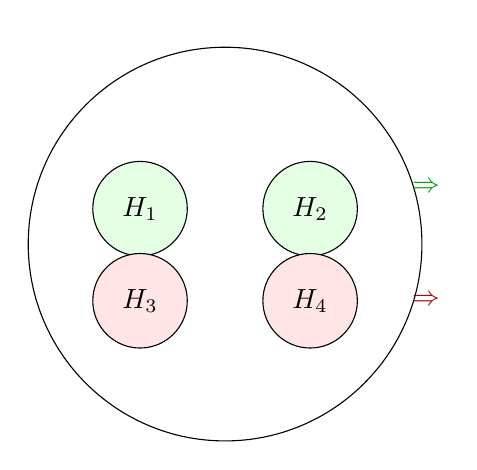
\begin{tikzpicture}[scale=0.9,
    subgroup/.style={draw,circle,minimum size=1.2cm,fill=blue!10},
    normsub/.style={draw,circle,minimum size=1.2cm,fill=green!10},
    nonnorm/.style={draw,circle,minimum size=1.2cm,fill=red!10}]
\node[draw,circle,minimum size=5cm,label=above:$\AuditGrp$] (G) at (0,0) {};
\node[normsub] (N1) at (-1.2,0.5) {$H_1$};
\node[normsub] (N2) at (1.2,0.5) {$H_2$};
\node[nonnorm] (NN1) at (-1.2,-0.8) {$H_3$};
\node[nonnorm] (NN2) at (1.2,-0.8) {$H_4$};
\node[anchor=west,text=green!60!black] at (2.5,0.8) { $\Rightarrow$ };
\node[anchor=west,text=red!60!black] at (2.5,-0.8) { $\Rightarrow$ };
\end{tikzpicture}
\caption{.（）;}
\label{fig:subgroup_structure}
\end{figure}
% ================================================================
% 8. Discussion
% ================================================================
\section{}
\subsection{}
CoreSCXGalois\textbf{awaiting}.
\begin{enumerate}[label=(\arabic*),itemsep=3pt]
    \item \textbf{} $\AuditGrp$ awaiting, Galois.
    \item \textbf{Galois}（~\ref{thm:galois_correspondence}）.
    \item \textbf{}（~\ref{thm:unsolvability}）Proof: $A_5 \leq \AuditGrp$ $\implies$ , .
    \item \textbf{}（~\ref{thm:normalizer}）Proof, , awaiting.
    \item \textbf{}（~\ref{thm:fixed_domain}）Proof$\CEC = \Fix(\AuditGrp)$.
    \item \textbf{-}（~\ref{thm:correlation_nonnormal}）.
\end{enumerate}
\subsection{SCXCore}
\begin{table}[htbp]
\centering
\caption{SCXCore}
\label{tab:theorem_integration}
\begin{tabular}{@{}p{3cm} p{5cm} p{5cm}@{}}
\toprule
\textbf{SCX} & \textbf{} & \textbf{（）} \\
\midrule
（Thm~3）&  & （~\ref{thm:unsolvability}）\\
（Thm~2）&  & $H \NotNormal \AuditGrp \iff$ （~\ref{thm:correlation_nonnormal}）\\
Situs Lipschitz & Lipschitz & （~\ref{thm:normalizer}）\\
\bottomrule
\end{tabular}
\end{table}
\subsection{——Honest Strike}
\honestcrit{？}
: $\ExpertSet$\textbf{}, $\AuditGrp$.
\begin{itemize}[itemsep=3pt]
    \item \textbf{}（）; 
    \item \textbf{}（GrowthDecays）; 
    \item \textbf{}（``''）.
\end{itemize}
\begin{enumerate}[label=(\arabic*),itemsep=3pt]
    \item \textbf{: }（）, Lie.Peter-Weyl.
    \item \textbf{profinite: }profinite, profinite, GaloisprofiniteVersion.
    \item \textbf{: }, .
\end{enumerate}
\honestcrit{？}
\begin{itemize}[itemsep=3pt]
    \item ``''\textbf{}（）; 
    \item \textbf{}（）; 
    \item \textbf{}（）.
\end{itemize}
\honestcrit{（$A_5$）？}
~\ref{thm:unsolvability}$A_5 \leq \AuditGrp$.
$A_5$60, , $A_5$？
, $\Sym_n$（$n \geq 5$）$A_5$（5）.
, \textbf{5}（$\Sym_5$）, $A_5$.
, \textbf{}: 
$A_5$\textbf{}, .
\subsection{}
\openproblem \textbf{Galois.} profinite.
\openproblem \textbf{.} $\AuditGrp$？
: \textbf{}.
\openproblem \textbf{Galois.} $H^1(\AuditGrp, \CEC)$``''？
\openproblem \textbf{Tannakian.} ``'', Tannakian？
SCX\textbf{}.
% ================================================================
% 9. Conclusion
% ================================================================
\section{Conclusion}
Core——$\AuditGrp$, Galois, , , 
\textbf{}, ``''——
% ================================================================
% References
% ================================================================
\begin{thebibliography}{99}
\bibitem{scx2026theorems}
SCX.
\emph{SCX Core Theorems: Honest Person, Strong Man, and the Foundations of Multi-Expert Auditing}.
Technical Report, 2026.
\bibitem{scx_causal}
SCX.
\emph{Causal SCX: Causal Inference}.
Preprint, 2026.
\bibitem{scx_lipschitz}
SCX.
\emph{Situs Lipschitz Decomposition for Multi-Expert Consensus}.
Technical Report, 2026.
\bibitem{scx_agentic}
SCX.
\emph{Agentic Multi-Agent SCX: Agentic Audit}.
Preprint, 2026.
\bibitem{scx_collective}
SCX.
\emph{Collective Intelligence SCX: }.
Preprint, 2026.
\bibitem{scx_information}
SCX.
\emph{Information-Theoretic SCX: }.
Preprint, 2026.
\bibitem{scx_temporal}
SCX.
\emph{Temporal SCX: }.
Preprint, 2026.
\bibitem{galois_classic}
E.~Galois.
\emph{M\'emoire sur les conditions de r\'esolubilit\'e des \'equations par radicaux}.
1846 (posthumous).
\bibitem{artin_galois}
E.~Artin.
\emph{Galois Theory}.
Notre Dame Mathematical Lectures, No.~2, 1944.
\bibitem{lang_algebra}
S.~Lang.
\emph{Algebra}, 3rd ed.
Springer, 2002.
\bibitem{serre_rep}
J.-P.~Serre.
\emph{Linear Representations of Finite Groups}.
Springer GTM 42, 1977.
\bibitem{szamuely_galois}
T.~Szamuely.
\emph{Galois Groups and Fundamental Groups}.
Cambridge University Press, 2009.
\bibitem{jacobson_galois}
N.~Jacobson.
\emph{Basic Algebra I}, 2nd ed.
W.H. Freeman, 1985.
\bibitem{dummit_foote}
D.~Dummit and R.~Foote.
\emph{Abstract Algebra}, 3rd ed.
Wiley, 2004.
\end{thebibliography}
% ================================================================
% Appendix
% ================================================================
\appendix
\section{Appendix:}
\subsection{}
\begin{definition}[]
$G$$\mathcal{L}(G)$$G$.
$H_1 \leq H_2$$\mathcal{L}(G)$$H_1 \subseteq H_2$（）.
\end{definition}
\begin{definition}[]
$N \leq G$\textbf{}, $N \Normal G$, $g \in G$, $g N g^{-1} = N$.
\end{definition}
\begin{definition}[]
$H \leq G$\textbf{}: 
\begin{equation}
    N_G(H) = \{g \in G \mid g H g^{-1} = H\}.
\end{equation}
$N_G(H)$$G$$H$.
\end{definition}
\subsection{Solvable Group}
\begin{definition}[Solvable Group]
$G$\textbf{}, 
\begin{equation}
    \{1\} = G_0 \Normal G_1 \Normal \cdots \Normal G_k = G,
\end{equation}
$G_i / G_{i-1}$Abel.
\end{definition}
\begin{definition}[Jordan-H\"older]
$G$\textbf{}, $G_i/G_{i-1}$.
\end{definition}
\begin{theorem}[Galois——]
$n \geq 5$, $S_n$., $S_5$$\{A_5, \Z/2\Z\}$, $A_5$.
\end{theorem}
\subsection{Galois}
$L/K$Galois, $G = \Gal(L/K)$.
\begin{theorem}[Galois]
\[
    H \mapsto \Fix(H) = \{x \in L \mid \forall \sigma \in H,\; \sigma(x) = x\}
\]
$\{\text{$G$}\}$$\{\text{$L/K$}\}$.
, $H \Normal G$$\Fix(H)/K$Galois.
\end{theorem}
\end{document}